\documentclass[11pt,a4paper]{article}
\usepackage{amsmath,amssymb,amsthm,graphicx,hyperref,booktabs,placeins}
\usepackage[margin=2.3cm]{geometry}
\newtheorem{theorem}{Theorem}
\newtheorem{proposition}[theorem]{Proposition}
\newtheorem{lemma}[theorem]{Lemma}
\newtheorem{corollary}[theorem]{Corollary}
\theoremstyle{definition}\newtheorem{definition}[theorem]{Definition}
\theoremstyle{remark}\newtheorem{remark}[theorem]{Remark}
\graphicspath{{../FIGURES/}}

\title{Finite daughter universes inside the domain of dependence of regular black holes}
\author{Project Baby Universe --- Genesis Branch\\ \small(version 2, for external review; not submitted)}
\date{1 November 2026}

\begin{document}
\maketitle

\begin{abstract}
In pure-gravity regularisations of black holes by quasi-topological curvature towers, collapsing matter bounces in a regular core.
Its continuation through the inner horizon is not determined by the field equations once perturbations make the Cauchy horizon a weak
null singularity. We show that a finite daughter does not need that continuation. For Oppenheimer--Snyder collapse we prove that an
interior event lies in the domain of dependence of the initial data if and only if $\eta+\chi<\eta_E+\chi_s$. Here $E$ is the point
where the ball's surface, after its bounce, reaches the inner horizon at advanced time $v=\infty$. In the de Sitter-core limit the
Cauchy-horizon cone reaches the daughter's centre exactly at conformal time $\pi/2$ after the bounce: the Cauchy horizon is the core's
de Sitter horizon. Large holes host a daughter that inflates for $N\simeq\ln C/(D-1)$ e-folds inside the domain. Compact,
near-threshold collapse in $D\ge7$ reaches its maximum and recollapses inside it. With the Dymnikova tower in $D=10$ the centre reaches
a second bounce; this is certified with margins up to $0.16$ against numerical errors of $10^{-11}$. A Lagrangian fluid code with a
Cauchy-horizon tracer, validated against the exact solution, shows that the cycle survives pressure and smooth inhomogeneity but not
strongly peaked central densities. Collider-formed holes, although near threshold, contain unbound massless matter and do not host the
daughter. We separate these new claims from established results.
\end{abstract}

\section{Introduction and what is established}
A closed world in place of the singularity of a black hole is an old idea: Markov's limiting curvature, and Frolov, Markov and Mukhanov
[PRD 41, 383 (1990)]. Bueno, Cano and Hennigar showed that infinite towers of quasi-topological densities in $D\ge5$ have regular black
holes as their unique spherically symmetric vacua [arXiv:2403.04827]. Thin-shell and Oppenheimer--Snyder collapse in these theories
bounce, and in the idealised geometry emerge through a white hole into a new region [arXiv:2412.02740, 2412.02742, 2505.09680]. Related
bounces arise in effective loop quantum gravity, where the horizon eventually disappears and the matter re-emerges [Kelly, Santacruz,
Wilson-Ewing, arXiv:2006.09325], and in toy models that match collapsing dust to an expanding FRW region at the price of
energy-condition violation [Chakrabarty et al., arXiv:1909.07129]. In the quantum Oppenheimer--Snyder hole, infall turns round inside
the Cauchy horizon [Idrissov, Quevedo, arXiv:2609.03278].

The obstacle is the inner horizon. Perturbations blueshift there (Poisson--Israel 1990; Ori 1991), and in these theories the Cauchy
horizon becomes a Tipler-weak null singularity in $D=5$ (our companion Paper A). Compact trapped regions avoid it semiclassically
[Carballo-Rubio et al., arXiv:2607.03916], but return the matter to the parent.

\textbf{What is new here} (to our knowledge; Section~\ref{sec:lit}):
\begin{itemize}
\item an exact characterisation of the domain of dependence of the bounced interior (Theorem~\ref{thm:dod});
\item the de Sitter timing law;
\item certified recollapse and full cycles inside the domain, with regime maps;
\item robustness under pressure and inhomogeneity;
\item a scope result excluding collider-formed holes.
\end{itemize}

\section{Setting and the daughter region}
Model U is $D=4+n$ dimensional gravity with the tower $h(\psi)$, $\mu=r^{D-1}h(\psi)$, in units $l=\sqrt\alpha=1$. We use the Hayward
tower $h=\psi/(1-\psi)$ and the Dymnikova tower $h=-\ln(1-\psi)$. A homogeneous dust ball of comoving radius $\chi_s$ has interior
$ds^2=a(\eta)^2(-d\eta^2+d\chi^2+\sin^2\!\chi\,d\Omega^2_{D-2})$ with
\[
\dot a^2=a^2\psi(a)-1,\qquad \psi=h^{-1}(C/a^{D-1}),\qquad C=\mu/\sin^{D-1}\chi_s .
\]
Every closed universe in these theories bounces at $a_b\ge l$. The exterior is $f(r)=1-r^2\psi(\mu/r^{D-1})$, with horizons $r_-<r_+$
for $\mu>\mu_{\rm ext}$. The initial slice $\Sigma$ is the moment of time symmetry, with the surface at rest at $R_0>r_+$ (untrapped
data).

\begin{definition}[daughter region and cycle]\label{def:daughter}
The bounce of a fluid worldline is where its expansion $\theta=\nabla\!\cdot u$ first turns from negative to positive. The daughter
region is
\[
\mathcal D=\{p\in D^+(\Sigma)\setminus J^-(\mathcal I^+):\ p \text{ lies on a fluid worldline after its bounce}\}.
\]
The stages along a worldline are: bounce; expansion; maximum ($\theta$ from $+$ to $-$); recollapse; second bounce. The daughter
completes a stage if an open neighbourhood of the centre reaches it inside $\mathcal D$. The size of a stage is the fraction of the
ball's proper volume that reaches it inside $\mathcal D$.
\end{definition}

\section{The domain of dependence}
\begin{lemma}[no turning point in the core]\label{lem:core}
$f$ decreases strictly on $(0,r_-]$. For Hayward, $f'=2\mu r\big(\tfrac{D-3}{2}r^{D-1}-\mu\big)/(r^{D-1}+\mu)^2$, and $r_-$ lies below
the minimum of $f$. For Dymnikova this is checked numerically.
\end{lemma}

\begin{theorem}\label{thm:dod}
An interior event $p=(\eta,\chi)$ to the future of $\Sigma$ lies in $D^+(\Sigma)$ if and only if $\eta+\chi<\eta_E+\chi_s$, where $E$ is
the post-bounce event at which the surface reaches $r=r_-$. All post-bounce interior events lie outside $J^-(\mathcal I^+)$.
\end{theorem}
\begin{proof}
\emph{(i) Reduction to the quotient.} By spherical symmetry, causal relations reduce to the $(t,r)$ quotient, with the centre as a
reflecting boundary. So $p\in D^+(\Sigma)$ iff both past radial null rays from $p$ meet $\Sigma$.

\emph{(ii) Interior rays.} In the interior these rays are $\eta\pm\chi=$ const. The ray towards the centre reflects and reaches the
surface before the other ray. The other ray reaches the surface at $\eta_S=\eta+\chi-\chi_s$.

\emph{(iii) The surface reaches $r_-$ only at $v=\infty$.} By Lemma~\ref{lem:core} the post-bounce surface has $\dot r\to E_s>0$ at
$r_-$, with $E_s^2=f(R_0)$. In ingoing Eddington--Finkelstein coordinates, $dv/dr\simeq2/f\simeq1/(\kappa_-(r_--r))$, so it reaches
$r_-$ only at $v=+\infty$, in finite proper time. Hence $E$ lies on $\{v=\infty\}$, and every earlier surface point has finite $v$.

\emph{(iv) Exterior continuation.} The ray towards the surface continues in the exterior as the ingoing null line $v=v_S$. For
$v_S<\infty$ this line, traced to the past, crosses $\Sigma=\{t=t_0\}$ at finite $r$, because $t=v-r_*\to-\infty$ as $r\to\infty$. For
a surface point after $E$, the line lies beyond the Cauchy horizon. That region contains past-inextendible causal curves that end at
the parent's timelike infinity without meeting $\Sigma$.

\emph{(v) Hidden.} Inside the ball the event horizon is $\eta-\chi=\eta_H-\chi_s$, with $\eta_H<\eta_b$ the inward crossing of $r_+$.
\end{proof}

\begin{remark}
Within spherical symmetry the reduced equations are hyperbolic while $h'(\psi)>0$, so the development in $D^+(\Sigma)$ is unique.
Uniqueness against non-spherical perturbations requires a well-posed formulation of the full tower, which is open. Mass inflation grows
only as $v\to\infty$, so points of $\mathcal D$ at finite distance from the cone see a bounded blueshift.
\end{remark}

\begin{proposition}[de Sitter timing law]
If $\psi\to1/\alpha$ near the bounce and $r_-\to\sqrt\alpha$, then $\cos(\eta_E-\eta_b)=\sin\chi_s$, so
$\eta_E+\chi_s-\eta_b=\pi/2$: the cone reaches the centre when the core's de Sitter phase would end. Numerically
$\eta_E+\chi_s-\eta_b\in[\pi/2,2.00]$.
\end{proposition}

\section{Certified cycles}
The stage times are computed with an ODE solver at three tolerances and with an independent quadrature. The error is the larger of the
two spreads. A stage is certified at the centre when $\eta_E+\chi_s-\eta_k$ exceeds ten times the error.
\begin{table}[h]\centering\small
\begin{tabular}{lccc}\toprule
$D$, tower, $\mu/\mu_{\rm ext}$, $\chi_s$ & maximum: $\chi$ (volume) & second bounce: $\chi$ (volume) & error\\\midrule
10, Dymnikova, 1.05, 1.4 & 0.873 (5.4\%) & 0.0566 ($2.5\times10^{-12}$) & $1\times10^{-12}$\\
10, Dymnikova, 1.01, 1.5 & 0.959 (7.7\%) & 0.1595 ($2.0\times10^{-8}$) & $7\times10^{-12}$\\
10, Dymnikova, 1.10, 1.4 & 0.831 (3.7\%) & 0.0083 ($8\times10^{-20}$) & $1\times10^{-12}$\\
10, Hayward, 1.20, 1.0 & 0.384 (0.05\%) & --- & $1\times10^{-12}$\\
10, Hayward, 1.05, 1.4 & 0.636 (0.46\%) & --- & $7\times10^{-12}$\\
5, Hayward, 20, 0.5 & --- & --- & $6\times10^{-11}$\\\bottomrule
\end{tabular}
\caption{Largest comoving radius whose stage event lies in $\mathcal D$, with the volume fraction of the ball it contains.}
\end{table}
The full-cycle window (Dymnikova, $D=10$) is $\mu\lesssim1.10\,\mu_{\rm ext}$ with $\chi_s$ from 1.26--1.39 up to about 1.55; it closes
at $\mu\approx1.13\,\mu_{\rm ext}$. In $D=9$ it survives only at $\mu\lesssim1.005\,\mu_{\rm ext}$. Because the $D=10$ volume element is
$\sin^8\!\chi$, the full cycle is completed only by a small central fraction of the ball. The maximum is reached by up to 7.7\%.

\section{Realistic matter in $D=10$}
\paragraph{Method.} We use the Lagrangian fluid code of our earlier work: generalised Misner--Sharp equations, pressure, tensor
viscosity, inelastic rezoning, and time equal to the proper time of the pressure-free surface. We extend it with four ingredients.
\begin{enumerate}
\item The event $E$, where the surface crosses $r_-(\mu)$ after its bounce. Outside the ball the exterior is static by Birkhoff's
theorem.
\item The Cauchy-horizon cone from $E$, traced through the fluid in the rest-mass coordinate. A zone of areal thickness $\Delta R$ has
proper thickness $\Delta R/\Gamma$; the ray covers proper distance $e^{\Phi}dt$.
\item Stage detection for tracked fluid elements. A maximum must re-expand the element by at least 2\% over its bounce radius, which
removes shock and pressure wiggles; the exact full-cycle case re-expands by 11\%.
\item Hiddenness. An event is counted only after the surface has crossed $r_+$. This is sufficient, because inside the matter the event
horizon reaches the surface at that time.
\end{enumerate}
The code reproduces the exact dust solution: cone arrival at the centre $2.6565$ against $2.658$, second bounce $2.6018$ against
$2.6008$. Verdicts are identical at $N=60,120,200$ zones.

\paragraph{Survey.} In $D=10$ we combine:
\begin{itemize}
\item four configurations: Dymnikova $(1.05,1.4)$, $(1.10,1.3)$; Hayward $(1.20,1.0)$, $(1.05,1.4)$ in $(\mu/\mu_{\rm ext},\chi_s)$;
\item five density profiles: uniform; cored $(1-x^4)^2$; parabolic $1-0.9x^2$; peaked $(1-x^2)^2$; Gaussian $e^{-3x^2}$;
\item four pressure levels: $\epsilon_0\in\{0,0.1,0.5,2\}$, i.e.\ central $p/\rho\le0.074$;
\item smooth density modes of 5\% amplitude (two seeds), or none.
\end{itemize}
Of the 240 runs, all form a black hole. 230 complete; 10 break down by shell crossing and are reported separately.
\begin{table}[h]\centering\small
\begin{tabular}{lcccc}\toprule
profile (completed runs) & full cycle & maximum + recollapse & expands, ends & no bounce in $\mathcal D$\\\midrule
uniform (48) & 12 & 36 & 0 & 0\\
cored, flat to $O(x^4)$ (48) & 0 & 25 & 21 & 2\\
parabolic (48) & 0 & 25 & 23 & 0\\
peaked $(1-x^2)^2$ (40) & 1$^*$ & 0 & 36 & 3\\
Gaussian (46) & 0 & 6 & 39 & 1\\\bottomrule
\end{tabular}
\caption{Verdict at the centre. $^*$Single run at the highest pressure; two of its three seeds broke down. Not counted as evidence.}
\end{table}

\paragraph{Findings.}
\begin{itemize}
\item \emph{Pressure and smooth inhomogeneity do not destroy the cycle.} With a homogeneous core, every run reaches its maximum and
recollapses inside $\mathcal D$, and a quarter complete the full cycle. Pressure up to $p/\rho\approx0.07$ slightly increases the
recollapsing fraction.
\item \emph{The central density gradient decides.} Profiles flat at the centre keep the maximum in about half the runs. Those with an
order-one quadratic central gradient mostly end while still expanding (75 of 86 completed runs): their central region re-expands later
than the cone arrives. The daughter needs a nearly homogeneous core.
\end{itemize}


\section{Formation channels: bound versus unbound content}
\begin{lemma}\label{lem:unbound}
Matter with $\Gamma>1$ (unbound; massless content is the limit $\Gamma\to\infty$) has $U^2=\Gamma^2-f>0$ throughout the core, where
$f\le1$, and never turns round there. A homogeneous unbound interior (open FRW) has $\dot a^2=a^2\psi+1>0$. It never bounces and reaches
$a\to0$ in finite proper time: a density caustic at bounded curvature.
\end{lemma}
At $\sqrt s=100$\,TeV ($n=6$, $M_D=8$\,TeV, $c_l=0.70$), produced holes have median $\mu/\mu_{\rm ext}=1.044$, with 80\% below 1.1. That
is the window of Section 4. But their content is two massless partons plus gravitational radiation, and the median spin is
$a_*\approx3.5$. By Lemma~\ref{lem:unbound} this content does not bounce: it streams through the core towards the Cauchy horizon.
\emph{Collider-formed holes do not host the bound daughter}; a collider discovery would test the curvature tower, not the daughter. The
daughter needs bound, compact, near-threshold collapse. We know no channel that provides it.

\begin{figure}[t]\centering
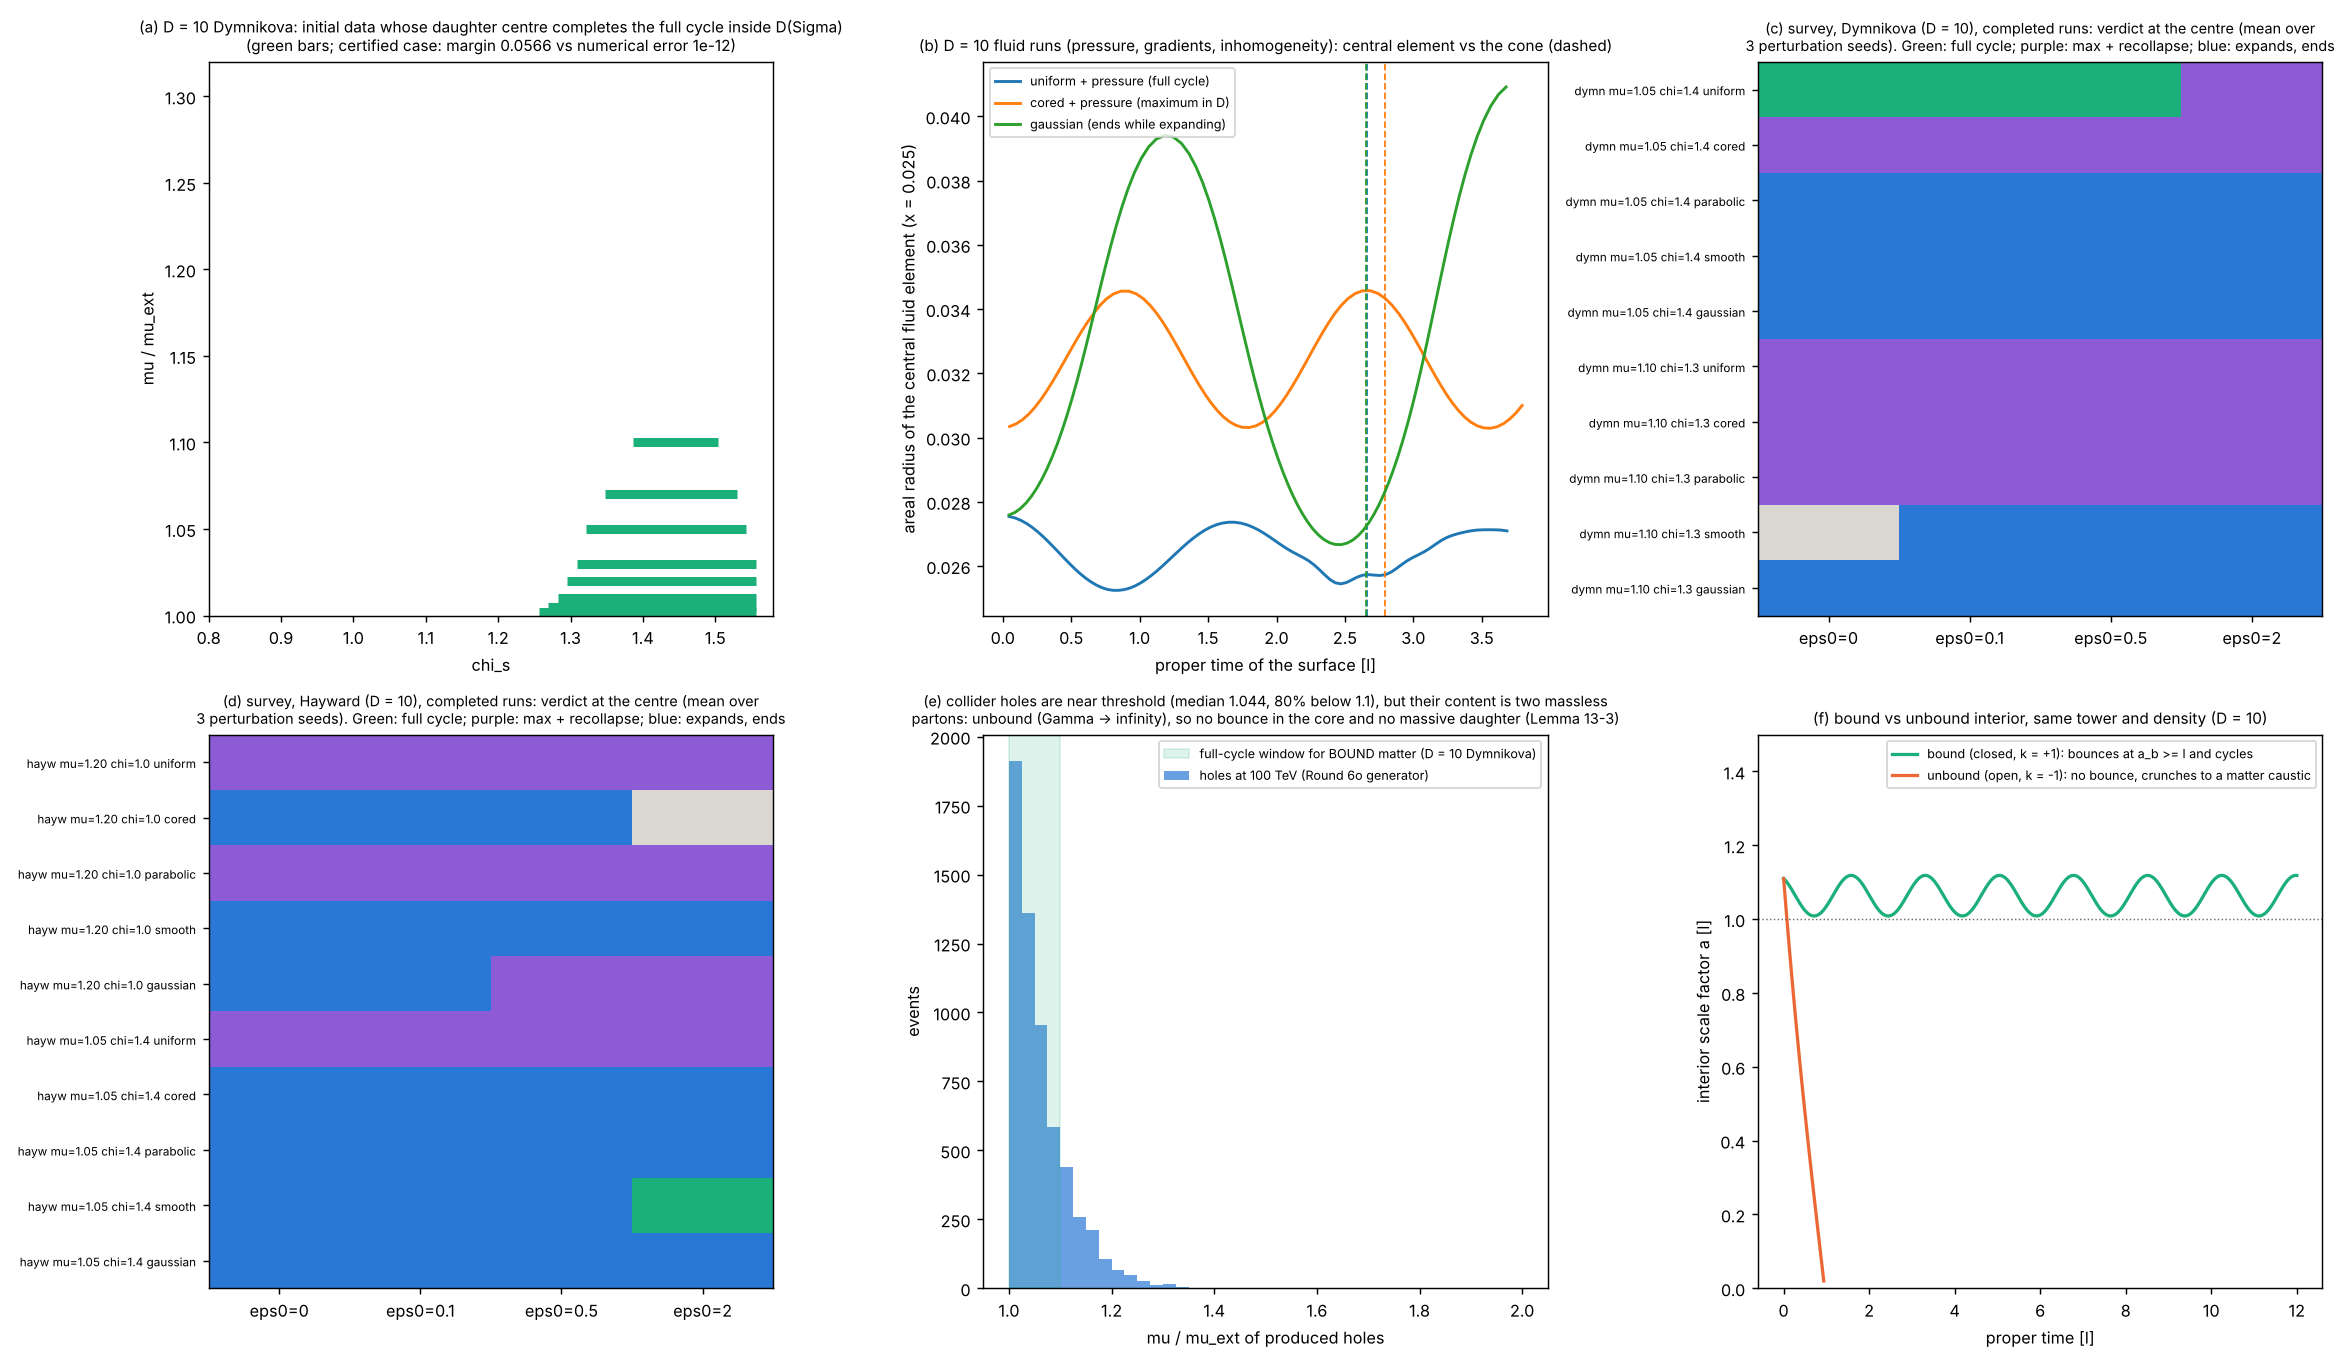
\includegraphics[width=\textwidth]{round13.png}
\caption{(a) Full-cycle window; (b) central fluid element against the Cauchy-horizon cone in three fluid runs; (c,d) survey verdicts;
(e) collider holes; (f) bound versus unbound interiors.}\end{figure}

\section{Relation to the literature}\label{sec:lit}
Frolov--Markov--Mukhanov and successors place a closed world inside the hole, by gluing or by limiting curvature, without dynamics for
the matter. Bueno et al.\ provide the field equations and the idealised extended geometry, in which the daughter lies beyond the inner
horizon. Effective loop-quantum-gravity bounces end with the matter returning to the parent. Our results sit between these: in a theory
with field equations, a finite daughter completes its cycle \emph{before} the Cauchy horizon, so neither a continuation prescription
nor a compact trapped region is needed. We found no prior treatment of the domain of dependence of the bounced interior, or of the
timing of the Cauchy-horizon cone against the daughter's cycle. A full-text search by referees is invited.

\section{Limitations}
\begin{itemize}
\item Spherical symmetry; uniqueness beyond it depends on the open well-posedness of the tower.
\item Dust and ideal-fluid matter only; no semiclassical back-reaction inside $\mathcal D$.
\item No rotation, and only a GR-scaling estimate for anisotropy.
\item The full cycle is reached by a tiny central volume fraction in $D=10$.
\item No known formation channel.
\item Nothing is claimed beyond the Cauchy horizon.
\end{itemize}

\section*{Reproducibility}
Branch \texttt{claude/bold-noether-qbcahe}, directory \texttt{genesis}. Run \texttt{CODE/scripts/round13.py} and
\texttt{round12.py}; data in \texttt{DATA/round13.json} and \texttt{round12.json}; tests in \texttt{CODE/tests/test\_round12.py} and
\texttt{test\_round13.py}; the proof in \texttt{ROUND13/CAUSAL\_DOMAIN\_PROOF.md}.

\section*{References}\small
Frolov, Markov, Mukhanov, PLB 216, 272 (1989); PRD 41, 383 (1990).
Bueno, Cano, Hennigar, PLB 861 (2025), arXiv:2403.04827.
Bueno, Cano, Hennigar, Murcia, arXiv:2412.02740, 2412.02742.
Bueno, Cano, Hennigar, Murcia, Vicente-Cano, arXiv:2505.09680.
Kelly, Santacruz, Wilson-Ewing, arXiv:2006.09325.
Chakrabarty, Abdujabbarov, Malafarina, Bambi, EPJC 80 (2020), arXiv:1909.07129.
Idrissov, Quevedo, arXiv:2609.03278.
Carballo-Rubio, Di Filippo, Liberati, Visser, arXiv:2607.03916.
Poisson, Israel, PRD 41, 1796 (1990). Ori, PRL 67, 789 (1991).
Gajic, Luk, arXiv:1709.09137. McMaken, PRD 107, 125023 (2023).
\end{document}
